\section{Minimal Structure: SSO}


\subsection{Why Two Layers Emerge: Grounding in Bio-IFGT}


Before entering this section, one point must be fixed.

The two-layer structure of fast and slow layers is not a distinction introduced for the convenience of explaining consciousness. This structure emerges necessarily from the process by which life attractors form.

Bio-IFGT describes life as a "dynamic quasi-closure structure created by information flow." For life to maintain a difference from its environment while sustaining itself, at least two processing operations at different time scales are required.

The first is fast processing, which handles immediate environmental response. It is involved in prediction, reaction, and error correction with respect to external change, and is volatile and rapid.

The second is slow processing, which retains successful response conditions for the next generation or next state. It is sedimentary and stable; structures once inscribed do not readily dissolve.

In Bio-IFGT simulation experiments tracing the hierarchical emergence path
$M \rightarrow \mathcal{I} \rightarrow N \rightarrow B \rightarrow E$
(morphogen field $\rightarrow$ information density $\rightarrow$ neural commitment $\rightarrow$ boundary stabilization $\rightarrow$ eye-like commitment), it has been confirmed that as structuring through information flow advances, fast exploratory flow and slow stabilizing structure spontaneously differentiate. These two time scales coexist while maintaining their difference, neither fully synchronizing nor fully separating.

This is not a coincidental coexistence. From the VED perspective, the persistence of difference that does not realize complete closure as an ordinary state is the driving force that generates structure, and the temporal difference between the two layers is the biological implementation of that driving force.

Accordingly, when this paper introduces SSO as the minimal temporal structure for consciousness, it stands on this biological two-layer differentiation. Consciousness is not a phenomenon that appears suddenly outside the life attractor; it is the state in which the difference maintained by life between fast response and slow retention has come to open a referencing relation.

With this accumulation in view, the following formalizes SSO as the minimal temporal structure for the establishment of consciousness.

SSO stands for Speed-Scale Orchestration.

It is a structure in which processing layers operating at multiple time scales are coordinated without central control.

In this paper, SSO is treated as the minimal temporal structure for the establishment of consciousness.

Crucially, SSO does not refer to any specific brain region.

SSO is not an anatomical structure.

It is a temporal arrangement that allows processes running at different speeds to continue interfering with each other without collapsing into synchrony or separating into disconnection.

\subsection{Two Minimal Layers}


As the minimal configuration, we consider at least two processing layers.

The first is the fast layer.

The fast layer is involved in prediction, forward models, momentary state updating, and immediate reaction.

Processing in this layer is rapid and volatile; most of it disappears without leaving a trace.

The second is the slow layer.

The slow layer is involved in storage, integration, memory sedimentation, and long-term structural change.

Processing in this layer is slow and stable; once a log has sedimented, it remains as a re-referenceable structure.

These two layers do not represent a difference in capability.

The fast layer is not superior and the slow layer inferior.

The difference between them lies in the temporal direction each faces.

The fast layer advances toward the future; the slow layer retains the past.

\subsection{Speed Differential}


The minimal condition for SSO is that the two layers are not running at the same speed.

Writing the speed of the fast layer as $v_f$ and the speed of the slow layer as $v_s$, the speed difference is:

\begin{equation}
\Delta v = v_f - v_s
\end{equation}

This speed difference is not an error.

It is, rather, the condition for SSO to obtain.

If $\Delta v = 0$, the fast and slow layers are fully synchronized, and no boundary arises between them.

Without a boundary, no referencing relation opens between current processing and past logs.

Therefore, at least the following condition is necessary for a conscious state to obtain:

\begin{equation}
\Delta v \neq 0
\end{equation}

However, a larger speed difference is not necessarily better.

If the speed difference is too large, the correspondence between the layers is lost and log referencing fragments.

What SSO requires is a finite speed difference that neither vanishes nor ruptures.

Figure~\ref{fig:sso} summarizes the minimal SSO structure.

\begin{figure}[H]
\centering
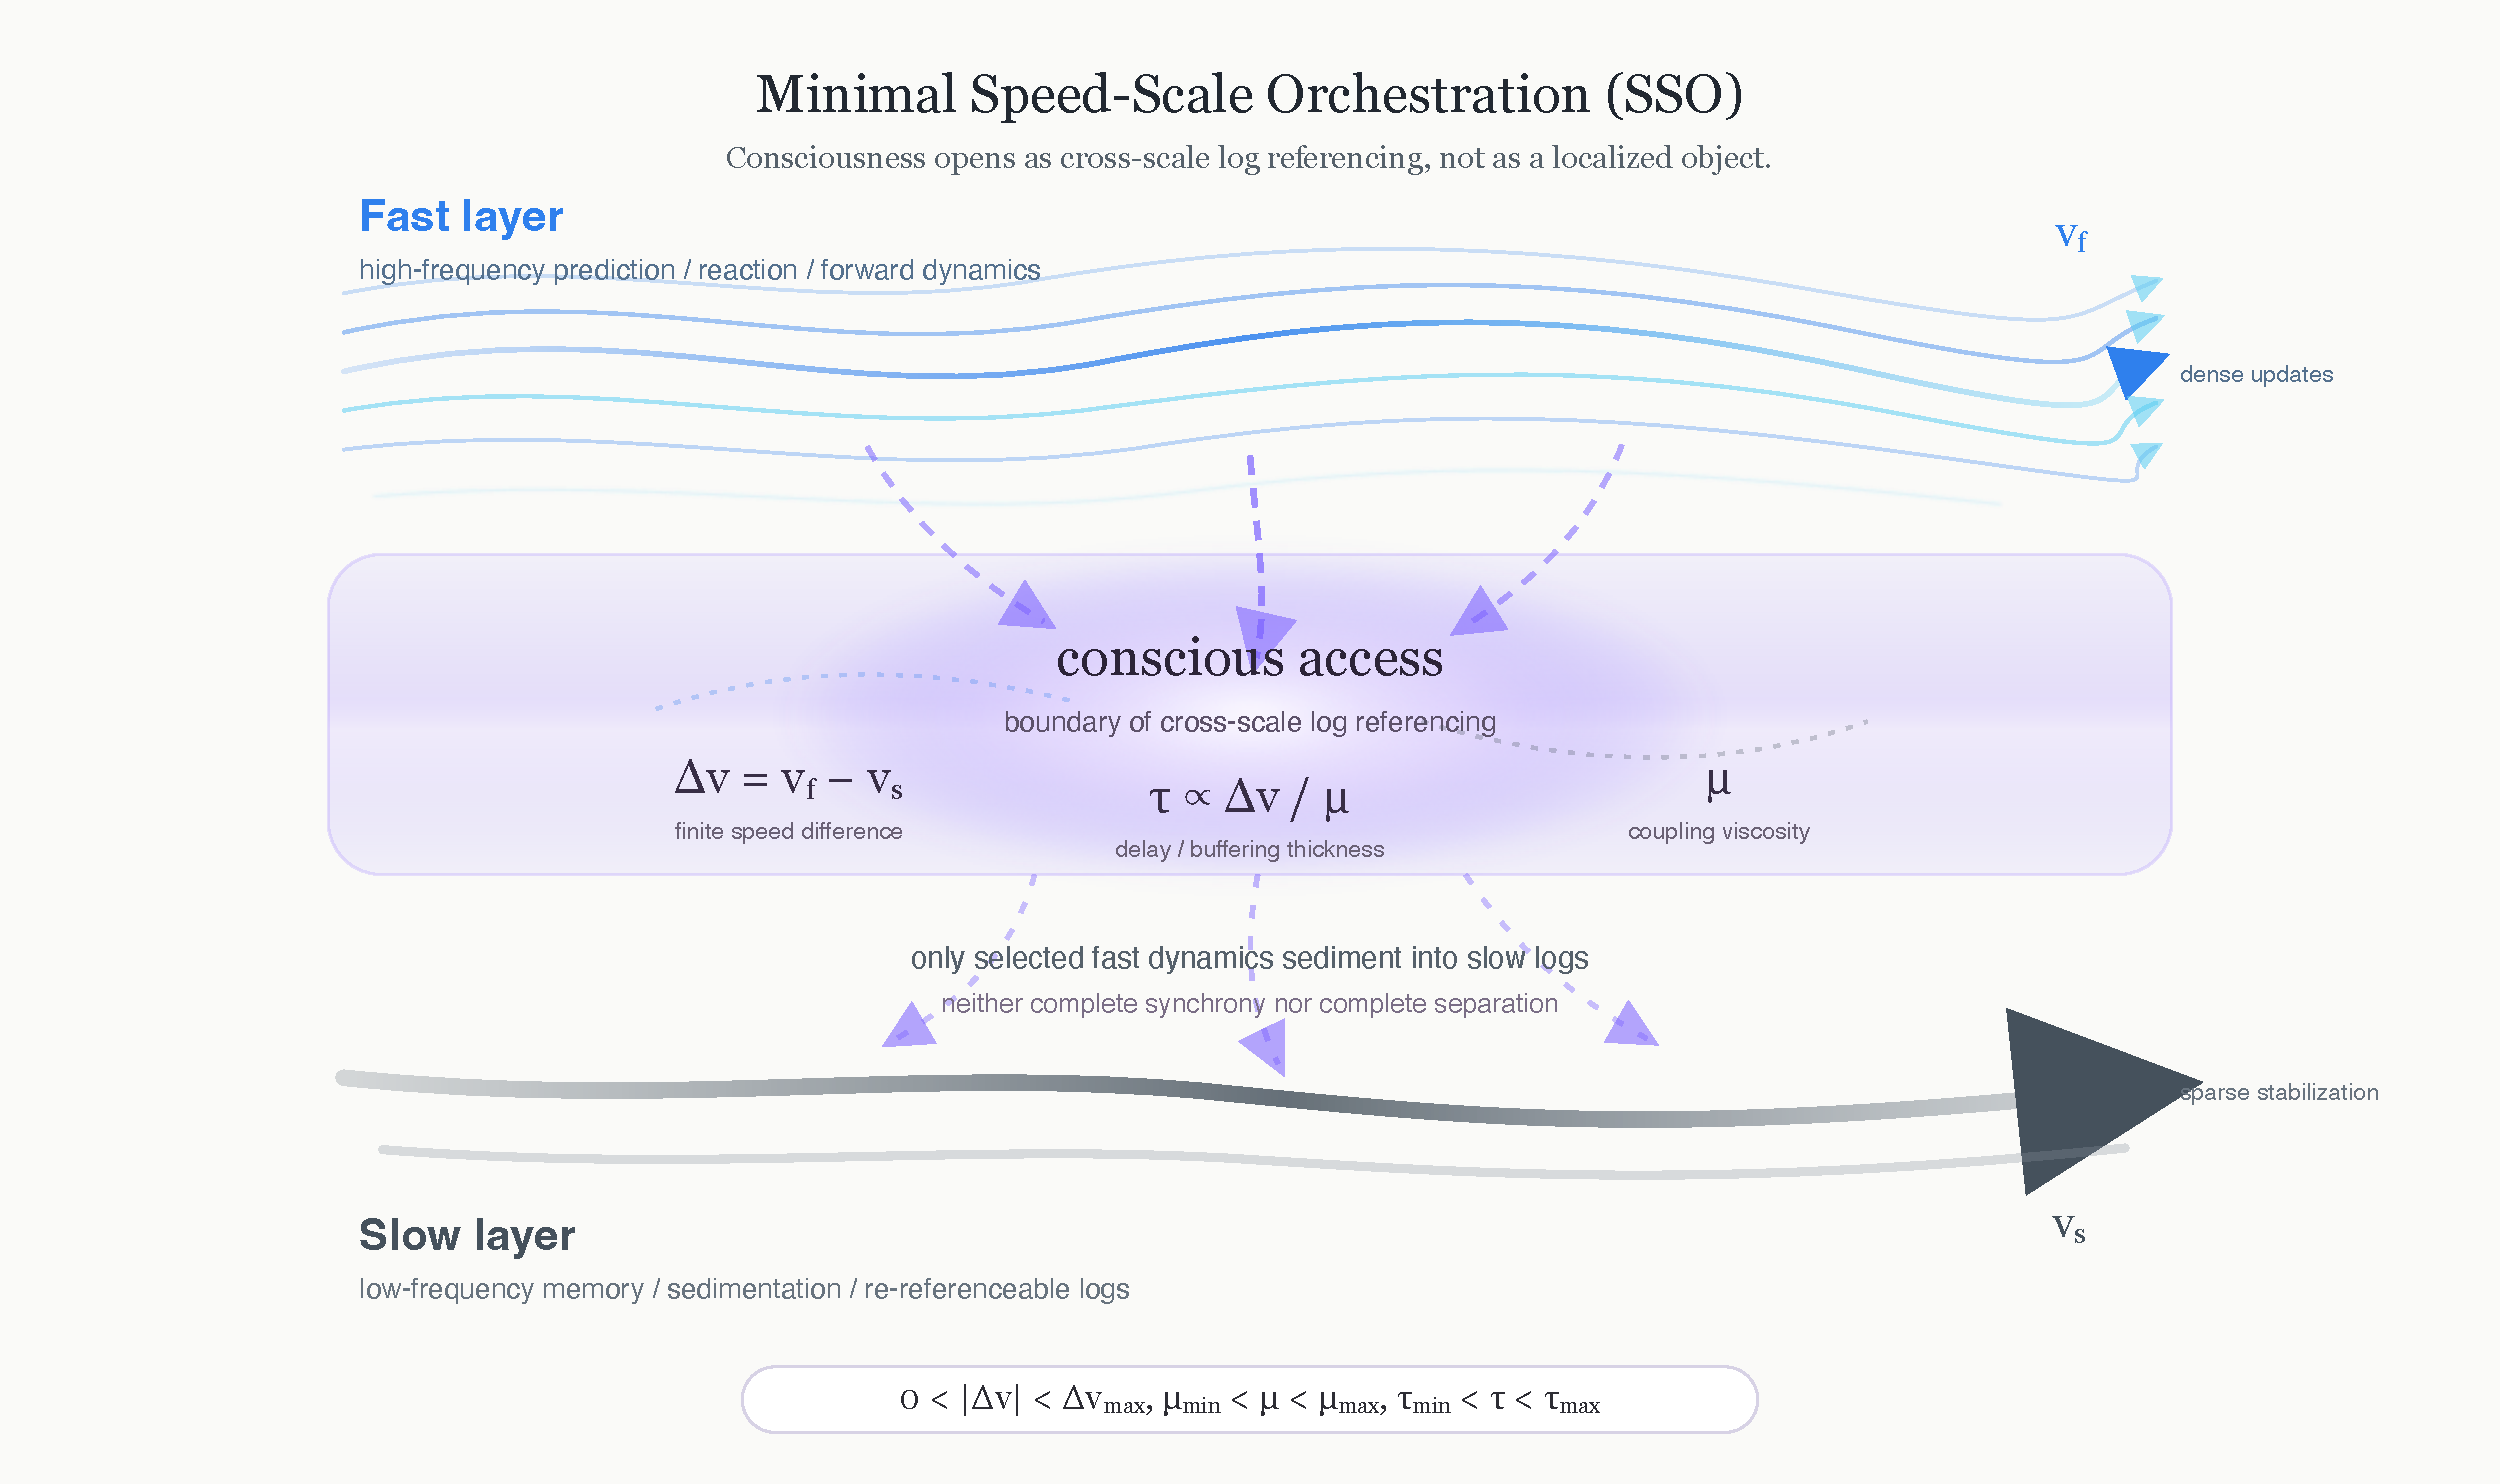
\includegraphics[width=0.92\linewidth]{figures/figure1_sso_density.pdf}
\caption{
Minimal structure of Speed-Scale Orchestration (SSO).
Consciousness is not localized in either the fast or slow layer, but opens at the boundary where fast predictive dynamics and slow sedimentary logs become mutually referenceable under finite speed difference, delay, and coupling viscosity.
}
\label{fig:sso}
\end{figure}

\subsection{Orchestration Without Control}


In SSO, no central controller governing the processing layers is assumed.

The fast layer does not dominate the slow layer, nor does the slow layer control the fast layer from above.

Both run independently at their respective time scales while interfering locally.

The term "orchestration" here does not mean control by a conductor.

It means that processes running at different speeds couple within a range that does not lead to breakdown, while preserving their mutual difference.

SSO is therefore coordination, not control.

More precisely, it is the retention of temporal asynchrony as a usable structure, without fully resolving it.

\subsection{Gate of Plasticity}


The interaction between the fast and slow layers requires a plasticity gate.

The plasticity gate does not determine what is processed.

It regulates whether the activity of the fast layer can modify the slow layer, and to what degree the structure of the slow layer constrains future fast processes.

If all activity of the fast layer were written into the slow layer, the system would become excessively rigid.

Conversely, if fast-layer activity never reached the slow layer, experience would not sediment and log referencing would not obtain.

The plasticity gate is therefore not an open/closed switch.

It is a temporal passage condition involving speed difference, delay, and viscosity.

Under this passage condition, only a portion of fast processing sediments into the slow layer and becomes a re-referenceable log.

\subsection{Internal Delay and Buffering}


In SSO, delay is not a defect.

Rather, it is because delay exists that a referenceable thickness arises between current processing and past logs.

This internal delay is written $\tau$:

\begin{equation}
\tau \propto \frac{\Delta v}{\mu}
\end{equation}

Here $\mu$ denotes the coupling viscosity between the fast and slow layers.

$\tau$ is not subjective time itself.

It is the internal time buffer during which processing that arose in the fast layer sediments into the slow layer and becomes referenceable as a log.

If $\tau$ is too small, processing flows away as immediate reaction and rarely becomes a referenceable log.

If $\tau$ is too large, the correspondence between current processing and log sedimentation breaks down and the conscious state fragments.

SSO is therefore not merely the coexistence of fast and slow processing.

It is a structure that maintains an appropriate delay range.

\subsection{SSO as Temporal Non-Closure}


From the VED perspective, SSO is a structure of temporal non-closure.

The fast and slow layers tend toward closure.

That is, processing tends to stabilize, sediment, and become fixed as a log.

But if closure is complete, the speed difference vanishes, flow stops, and the boundary of consciousness is lost.

Conversely, if there is no closure, processing flows away and does not remain as a log.

SSO lies between these two extremes.

It tends toward closure but does not close completely.

It tends toward separation but does not sever completely.

Within this non-closed temporal structure, a referencing relation opens between current processing and past logs.

In this sense, SSO is not a device that generates consciousness.

SSO is the temporal condition under which consciousness can open.

\begin{quote}
\textbf{Correspondence with CT (Conceptual Topography §2.4):} In Conceptual Topography, the $\Phi$ landscape formed by the slow layer is described as "an invisible GPU operating below the threshold of conscious access." Thought flows across the terrain, but the terrain itself is not directly referenced by consciousness. The fast/slow layer difference in this paper appears in CT as the asymmetry between "the visible flow ($J_I$) and the invisible landscape ($\Phi$)." Returning to this section after reading CT reveals that the temporal conditions of SSO share the same structure as the formation conditions of the conceptual landscape.
\end{quote}

\subsection{From SSO to Self-Sustaining Observer}


SSO was introduced as Speed-Scale Orchestration.

But when this structure forms a stable temporal loop, the same structure can be read as a Self-Sustaining Observer.

Here, "observer" does not mean a subject contemplating the world.

It refers to a structure in which current processing, past logs, and the plasticity gate form a mutually non-closed loop and self-sustainingly maintain a referencing state.

The fast layer anticipates the future.

The slow layer retains the past.

The plasticity gate regulates what sediments and what flows away between the two.

When this loop stabilizes, the system can update its state by referencing its own logs without external control.

This is where observer-like character appears.

However, this is not because a subject has been added.

It is simply that the temporal structure has become self-sustaining.

\subsection{Minimal Conditions}


Summarizing the above, the minimal conditions for SSO to obtain can be organized as follows:

\begin{enumerate}
\item Fast and slow layers exist.
\item There is a finite speed difference $\Delta v$ between them.
\item The speed difference does not reach either complete synchrony or complete separation.
\item A plasticity gate allows some portion of processing to sediment into the slow layer.
\item Internal delay $\tau$ is maintained as referenceable temporal thickness.
\item This structure forms a self-sustaining loop without central control.
\end{enumerate}

When these conditions are met, the system is not merely a processing device but possesses a temporal structure capable of log referencing.

This structure itself is not yet consciousness.

But without this structure, consciousness cannot obtain.

The next section introduces Torque Converter Attention as the mechanism that transforms speed differences within this SSO without rupture.
